%!TEX TS-program = xelatex
\documentclass{article}
\usepackage{amsmath}
\usepackage{lineno}
\usepackage{leftidx}
\usepackage[draft]{todonotes}
\usepackage{soul}
\usepackage{setspace}
\usepackage{fontspec}
\usepackage{graphicx}
\usepackage{pgfplotstable}
\usepackage[citestyle=numeric, sorting=none]{biblatex}
\addbibresource{tex.bib}
\setmainfont[Ligatures=TeX]{Ubuntu}
\setsansfont[Ligatures=TeX]{Ubuntu}
\renewcommand{\baselinestretch}{2.0}
\linenumbers
\fontdimen2\font=7pt
%content
\begin{document}
\title{Algorithmic detection of lateral gene transfer using regression
analysis}
\author{Alexander I Tuzhikov, Valery I Shestopalov,
Yuri V Panchin, Alexander Y Panchin}
\date{\today}

\maketitle
\linenumbers
\section{Abstract}
\subsection{Background}
Genes within a single genome may have different phylogenetic histories: most
genes were passed down ``vertically'' from the direct ancestors of the
organism, while others may have been acquired via horizontal gene transfer
(HGT) from other species. HGT is common between prokaryotes, but has been
observed between prokaryotes and eukaryotes, and even between different
eukaryotic species. Such events may lead to substantial evolutionary
consequences. However, no consensus has been reached neither on the necessary
criteria required to confirm HGT, nor about the scale on which HGT may occur
outside the prokaryotic domains of life.
\subsection{Results}
We propose a novel regression analysis based approach to identify putative HGT
events in genomic sequences. Using this technique we confirmed some of the
previously reported cases of HGT (such as the transfer of ankyrin-encoding
sequences from eukaryotes to their symbiotic bacteria or the acquisition of
thaumatin by Caenorhabditis) and predicted a number of novel candidates for HGT
(such as the putative acquisition of MaoC dehydratase domain containing
proteins by Lokiarchaeota).
\subsection{Conclusions}
Our approach may be useful to discover candidate sequences with
``non-vertical'' phylogenetic histories, implicated in HGT.
\todo{I am not sure is we want to have this ``limitation'' thing here..}
Limited by the computational complexity of the algorithm described here, we
were able to compare only a moderate number of smaller genomes. Larger studies
however will improve the recall and coverage leading to further HGT event
discoveries.

\section{Introduction}
\label{intro}
Horizontal gene transfer (HGT) is widely accepted as an important factor in the
evolution of prokaryotic organisms \cite{Ochman2000}. At the
domain-of-life-scale, a number of HGT events between prokaryotes and
eukaryotes, and even between different eukaryotic species have been described
[needs link], and in some cases have revealed molecular mechanisms that
facilitate transmission \cite{Soucy2015}. For example, agrobacteria are widely
used in modern biotechnology because of their natural ability to transfer some
of their genes horizontally into plant genomes \cite{Chilton1977}. Plants with
genes of bacterial origin are thus not uncommon \cite{Kyndt2015, Matveeva2012,
Matveeva2014}. Another peculiar case is the acquisition of genes by arthropods
from bacterial endosymbionts. For instance, the genome of the
\textit{Callosobruchus chinensis} beetle contains around 30\% of the
\textit{Wolbachia} genome \cite{Nikoh2008}. Viruses may also contribute to
lateral gene transfer \cite{Drezen2017}. A particular gene of retroviral origin
encoding a protein called ``syncytin'' plays an important role in mammalian
placenta morphogenesis \cite{Mi2000}. There is some evidence that HGT can occur
between different eukaryotic species \cite{Soucy2015}, for example between
certain parasitic plants and their hosts
\cite{Yoshida2010,Xi2012,Zhang2013,Zhang2014}, but overall our knowledge of
this field is scarce. There is ongoing controversy about the extent to which
HGT plays a role in eukaryotic evolution. Numerous examples of HGT were found
in different eukaryotic species, including humans by Crisp et al
\cite{Crisp2015}. However, other researchers failed to confirm some of the
published HGT findings \cite{Salzberg2017}. A study by Ku et al concluded that
even the gene transfer from bacteria to eukaryotes happens only occasinally and
coincides with major evolutionary transitions such as the origin of
chloroplasts and mitochondria \cite{Ku2015}. It should be noted that Ku et al
analyzed eukaryotic gene families with prokaryotic homologs and used clustering
and phylogenetic analysis. Crisp et al used differences in blast bit-scores
between prokaryotic and non-prokaryotic best hits of eukaryotic genes as a
criterion for the identification of the putative HGT events. Thus, these
studies are quite different by design, including the formulated requirements
for HGT. Remarkably, the scientific community is yet to decide what may
constitute sufficient evidence to consider a gene to have been obtained through
an HGT event. Here we present a novel regression-based approach for the
identification of candidate HGT events in genomic sequences, and report our
findings of putative HGT events in 61 genomes covering different branches of
the tree of life.

\section{Methods}
\subsection{Genomes and protein-coding regions used}
We used publicly available nucleotide sequences of 61 genomes from major
domains of life (Supplement 1). Since these genomes have varying annotation
depth, we adhered to a heuristic approach and analyzed each genome for open
reading frames of minimum length 150 b.p. as proxies to encoded putative
protein sequences (PPS). These regions may or may not correspond to existing 
genes, because splicing was not taken into account.
\todo{Meh...}
\hl{We did not use any of the
existing annotations so that well-annotated and poorly annotated genomes were
handled in the same way, and no bias corresponding to the different annotation
processes used by different authors could have influenced our results. That way
we also did our best not to miss any of the non-annotated protein-coding
sequences.}
As a result, for each genome considered we created a set of PPSs.

\subsection{Similarity search and normalization}
\label{simsearch}
Let $G_A, G_B$ denote genomes $A$ and $B$ respectively, and let a ``genome'' be
a finite set of all possible PPSs that can be derived from its nucleotide
sequence (the length of a PPS in this study is subject to constraints $150 \leq
length(PPS) \leq 1e4$):

\begin{equation}
G_A = \{g_A^1, g_A^2, \ldots, g_A^{L_A}\} = \{g_A^i\}_{i=1}^{L_A}
\end{equation}
where $g_A^i$ is a PPS from genome $A$ with index $i$, $L_A$ is the size of
the genome-set $A$.
Should we choose to search the most similar sequence for some $g_A^i$ in some
$G_B$ using a BLASTP algorithm implementation, we will end up with a (possibly
empty) set of best hits (empty if no significantly similar sequence could be
found in the reference set). If the hit set is not empty, we would be
interested in the topmost hit and its bit-score denoted $b_{A \rightarrow
B}^i$. More formally:

\begin{equation}
B(g_A^x, G_B) = BLASTP(g_A^x, G_B)=\left \{
\begin{aligned}
&b_{A \rightarrow B}^i\\
&0, && \text{if no hits found}
\end{aligned} \right.
\end{equation}

Suppose now that we are provided with a finite set of genomes \\
$S = \{G_1, G_2, \ldots, G_M\} = \{G_j\}_1^M$, where $M$ is the number of
genomes in the set (61 total in this study). Should we choose to search for
sequence similarity for some $g_A^x$ in each genome, we will assemble a
vector of best hit bit-scores:

\begin{equation}
V_{g_A^x} = (B(g_A^x, G_1), B(g_A^x, G_2), \ldots, B(g_A^x, G_M)) = (B(g_A^x,
G_j)_{j=1}^M)
\end{equation}

Obtained for each $g$ in every $G$ and ``stacked'' together, the $V$ vectors
form a matrix $BM$ of size $N*M$, where $N=\sum_{i=1}^k L_{G_i}$ and $M$,
again, -- the total number of genomes in the study.
\todo{need an illustration here}
For further analysis we chose
to ``filter'' $BM$ to only include $V$s which had at least 3 distinct hits
(``distinct'' here means the bit-score of a similarity search $B(g_A^x,
G_B)>0$), and denote such ``filtered'' matrix: $BM^+$.

As the last step of the data preparation we suggested that the bit-score values be
scaled as follows. $b_{A \rightarrow A}^x = B(g_A^x, G_A)$ is essentially a
result of a search for the best hit for $g_A^x$ within genome $A$, which is
$g_A^x$ itself, and the bit-score of such a match is the maximum possible for
the given $g_A^x$. We will thus perform the scaling as for each $b$ in $BM^+$:

\begin{equation}
\leftidx{^0}b_{A \rightarrow B}^x = \dfrac{b_{A \rightarrow B}^x}{b_{A \rightarrow
A}^x}
\end{equation}

\newcommand{\bmzp}{\leftidx{^0}BM^+}

and the resulting scaled matrix we denote $\leftidx{^0}BM^+$. This matrix and
its slices, corresponding to $g$s from individual subsets of genomes, we will
be using for further analysis (see Attachment).

The matrix $\bmzp{}$ obtained above will be used for pairwaise genome
comparison with the following general approach:
for each pair of $G \in S$ (denote a pair of some genomes $A$, $B$ as
$P_{A,B}$) a ``slice'' of the matrix $\bmzp{}$
will be obtained (denote $Slice_{A,B}$), which means that for a $P_{A,B}$ we
will select a submatrix of $\bmzp{}$ with all columns except for those
corresponding to $A$ and $B$ and rows corresponding only to $A$ and $B$ (denote
$\leftidx{^0}BM_{A,B}^+$).
\newcommand{\bmzpab}{\leftidx{^0}BM_{A,B}^+}
\todo{Need an illustration here}
We will then fit a logistic regression model using the {\tt glm{()}} funciton
in R with the {\tt family=} parameter set to {\tt "binomial"}. The model will
then be reduced to a minimal with {\tt step()} with {\tt direction="both"}. The
reduced model will be used to bootstrap the $\beta$ coefficients of the model
with {\tt boot()} and a custom function provided for sampling (see Attachment).
In essense, the sampling function achieves the following: vectors from the
reduced data matrix are sampled with replacement, a sampled matrix is used to
fit a new logistic regression model, and the $\beta$ coefficients for
predictors of the new model are retained. Finally, the median $\beta$
coefficient for each predictor across all training iterations (1000 in this
study) is selected to assemble a final ``bootstrapped''
model. The bootstrapped model will be used to assign probabilities for each
vector within $\bmzpab$ matrix (and thus $g$ from $A$ and $B$) to ``likely
belong'' to $A$ or $B$ respectively.

As a minor digression, we would like to discuss the possible states of a $g$
after it has been classified by the bootstrapped model. Should some $g_A$ be
assigned to cluster $A$ by the logistic regression model, we call such $g$
a $g$-``core''. Conversely, a $g_A$ assigned to $B$ is a $g$-``outsider''. As
regarding the term ``assigned'' above: denote the first case probability as $P(g_A \in
A)$. In order to confidently ``assign'' $g_A$ to genome $A$, we chose a margin
$P(g_A \in A) >0.975$, and a $g_A^x$ is called $g_A^x$-core only if $P(g_A^x
\in A) > 0.975$ in accordance to the bootstrapped logistic regression model.
Furthermore, a $g_A^x$ is called $g_A^x$-outsider if $P(g_A^x \in A) < 0.025$,
which would indicate that $g_A^x$ is far more likely to be coming from $B$,
than from its true origin - genome $A$. It is clear that for many $g_A$ $0.025
< P(g_A \in A) < 0.975$ will hold. We call such $g_A$ ``uncertain'', and
speculate that the number of such $g$ is likely to decrease with the addition
of new genomes to the input set, thus increasing the resolution of the method.


\section{Results and discussion}
\label{rad}
\subsection{Outsider detection}
\label{outsider_detection}
We built 61*60/2 = 1830 bootstrapped regression models to analyze a total of
296639 distinct PPS. A total of 67\% of the trained regression models passed
model quality control. Let us use the \textit{Drosophila
simulans}/\textit{Wolbachia} pair as an example of what was done. Figure
~\ref{fig:pca_analysis} shows a principal component analysis (PCA)
visualization of sequence clustering based on the normalized values of bit
scores for the \textit{Drosophila simulans} and \textit{Wolbachia} metagenomic
experiment. A clear separation of sequences can be observed even without the
use of regression analysis by PCA alone; however, we used PCA analysis only for
illustrative purposes.
\begin{center}
\begin{figure}
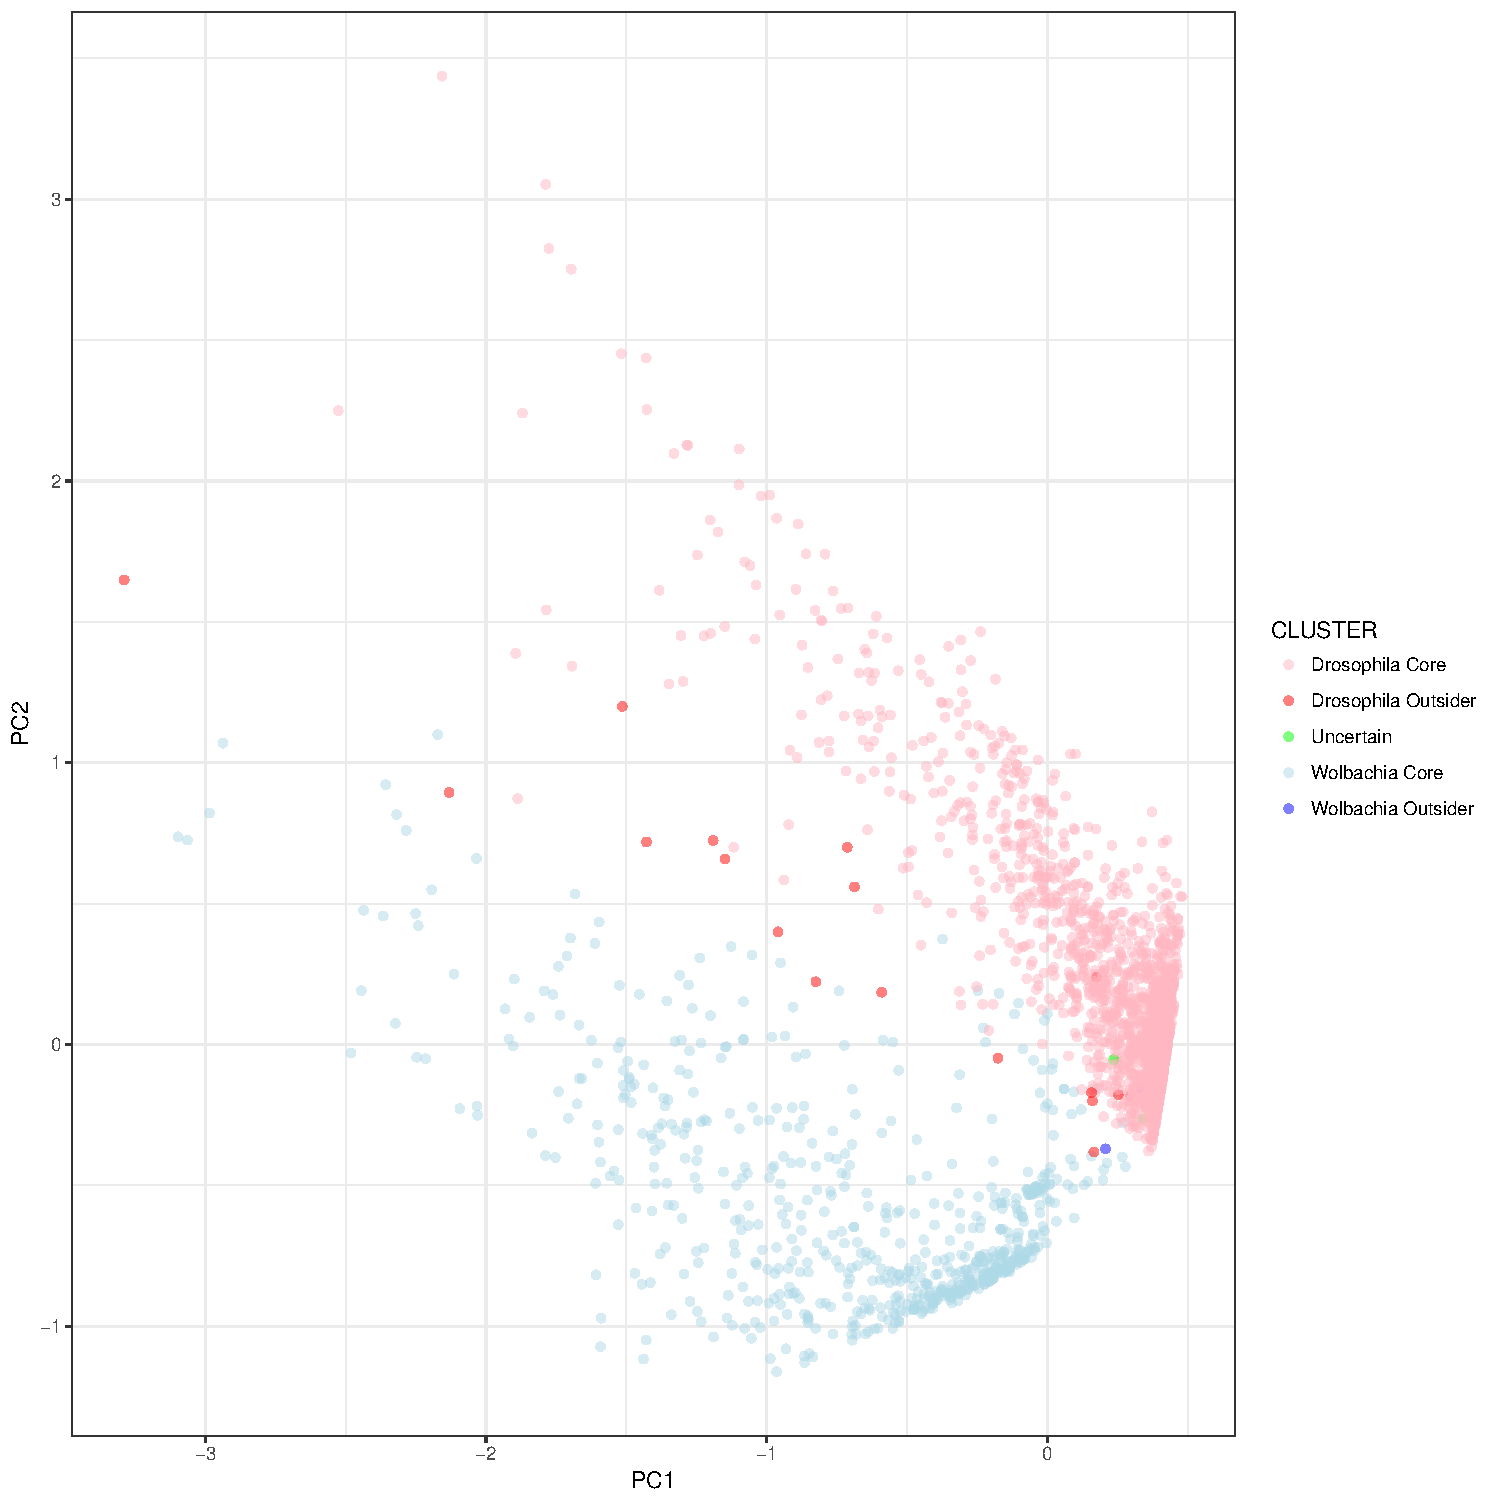
\includegraphics[width=12cm]{figures/w_eds_vs_ds_bootstrapped_pc1_pc2.pdf}
\caption{PCA analysis for clusters of predicted \textit{Drosophila simulans}
	and \textit{Wolbachia PPS}.}
\label{fig:pca_analysis}
\end{figure}
\end{center}
Figure ~\ref{fig:rsquared_barplot} contains an overview of the regression
models for \textit{Drosophila simulans} and each genome it was compared with.
Core genes are PPS from a genome that were correctly assigned to that
particular genome by the regression analysis. Outsider PPS are sequences that
were assigned to the other genome. The uncertain PPS are marked gray.
\begin{center}
\begin{figure}
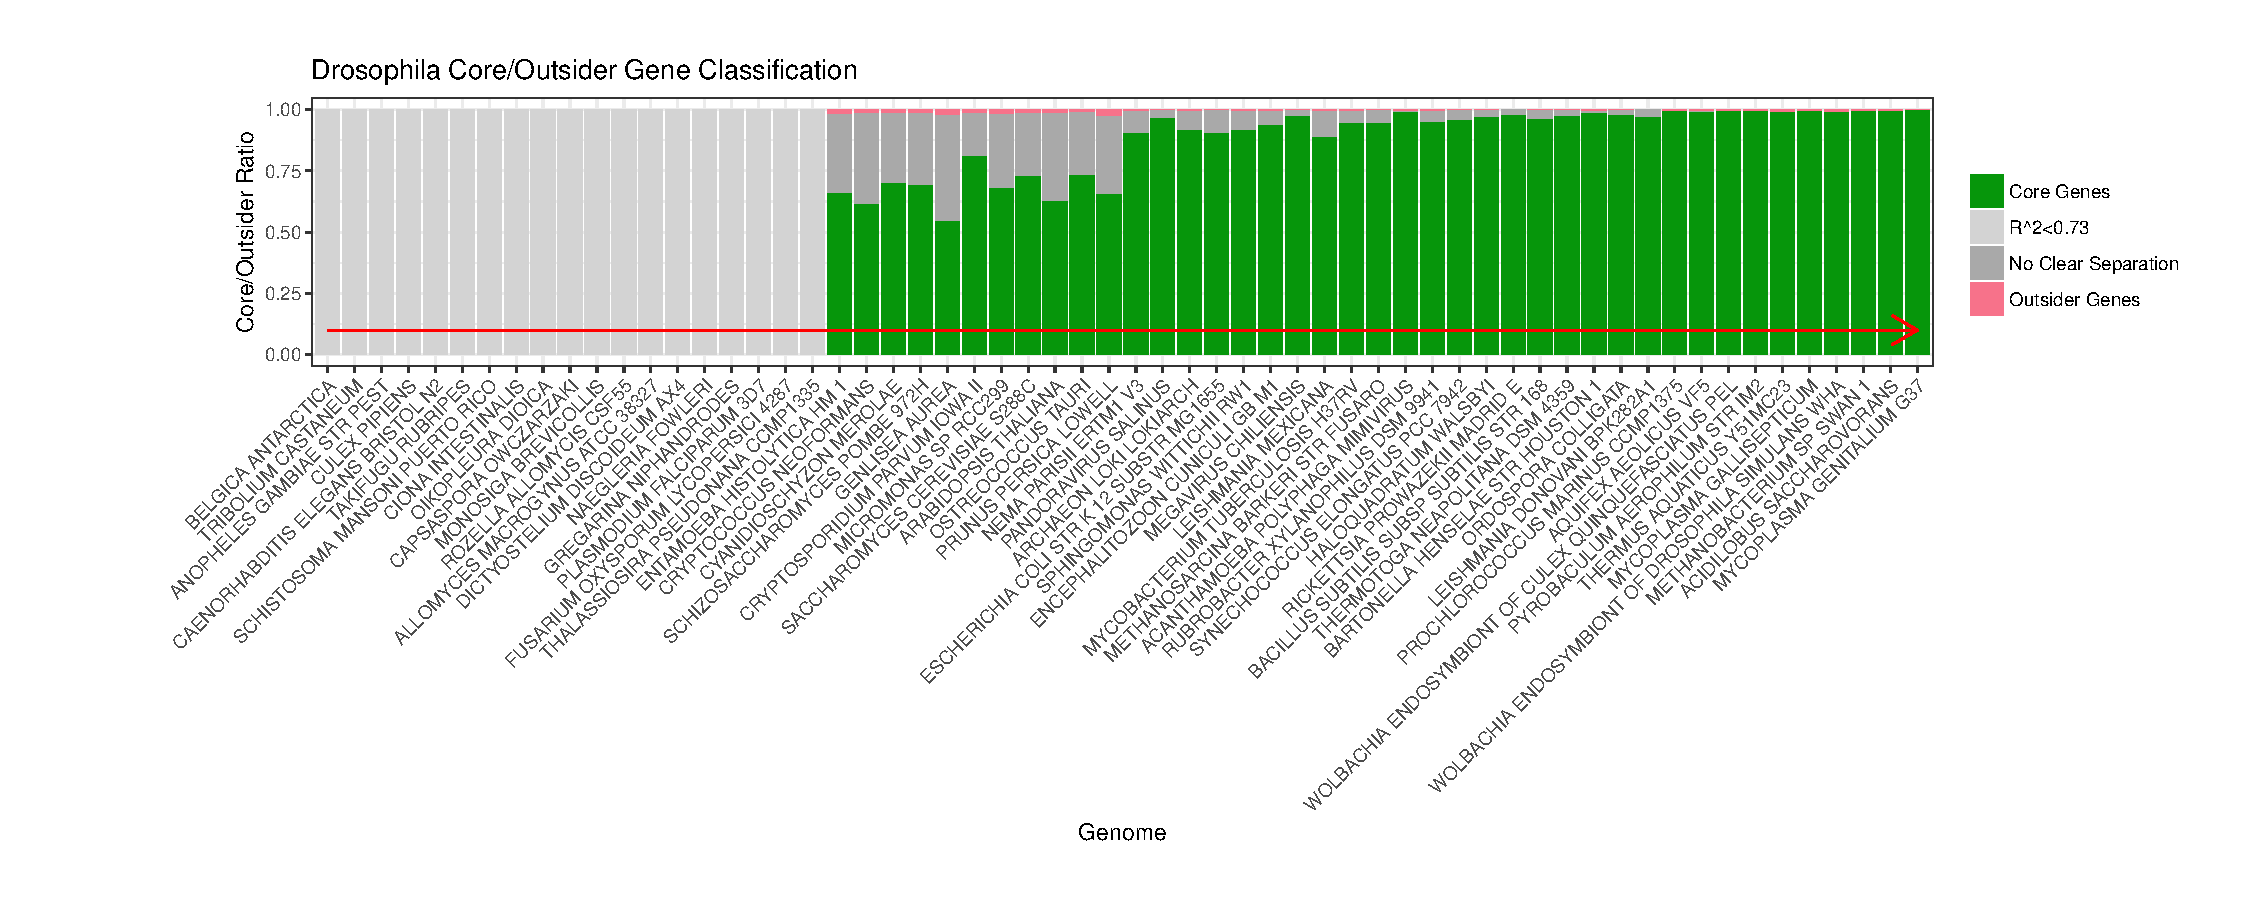
\includegraphics[width=12cm]{figures/core_outsider_barplot_bootstrapped.pdf}
\caption{The fraction of core/outsider \textit{Drosophila simulans} genes in
each model. The gray coloring represents the genome pairs where separation of
genes was not successful ($R^2$ < 0.73)}
\label{fig:rsquared_barplot}
\end{figure}
\end{center}

Figure ~\ref{fig:rsquared_curve} presents the $R^2$ values obtained for
regression models using \textit{Drosophila simulans} and each other genome in
our dataset (higher $R^2$ values are better). As expected, it is difficult to
separate the sequences of closely related arthropods (low $R^2$ values) but
it is easy to fulfill this task for distantly related genome pairs such as
\textit{Drosophila} and \textit{Mycoplasma}.
\begin{center}
\begin{figure}
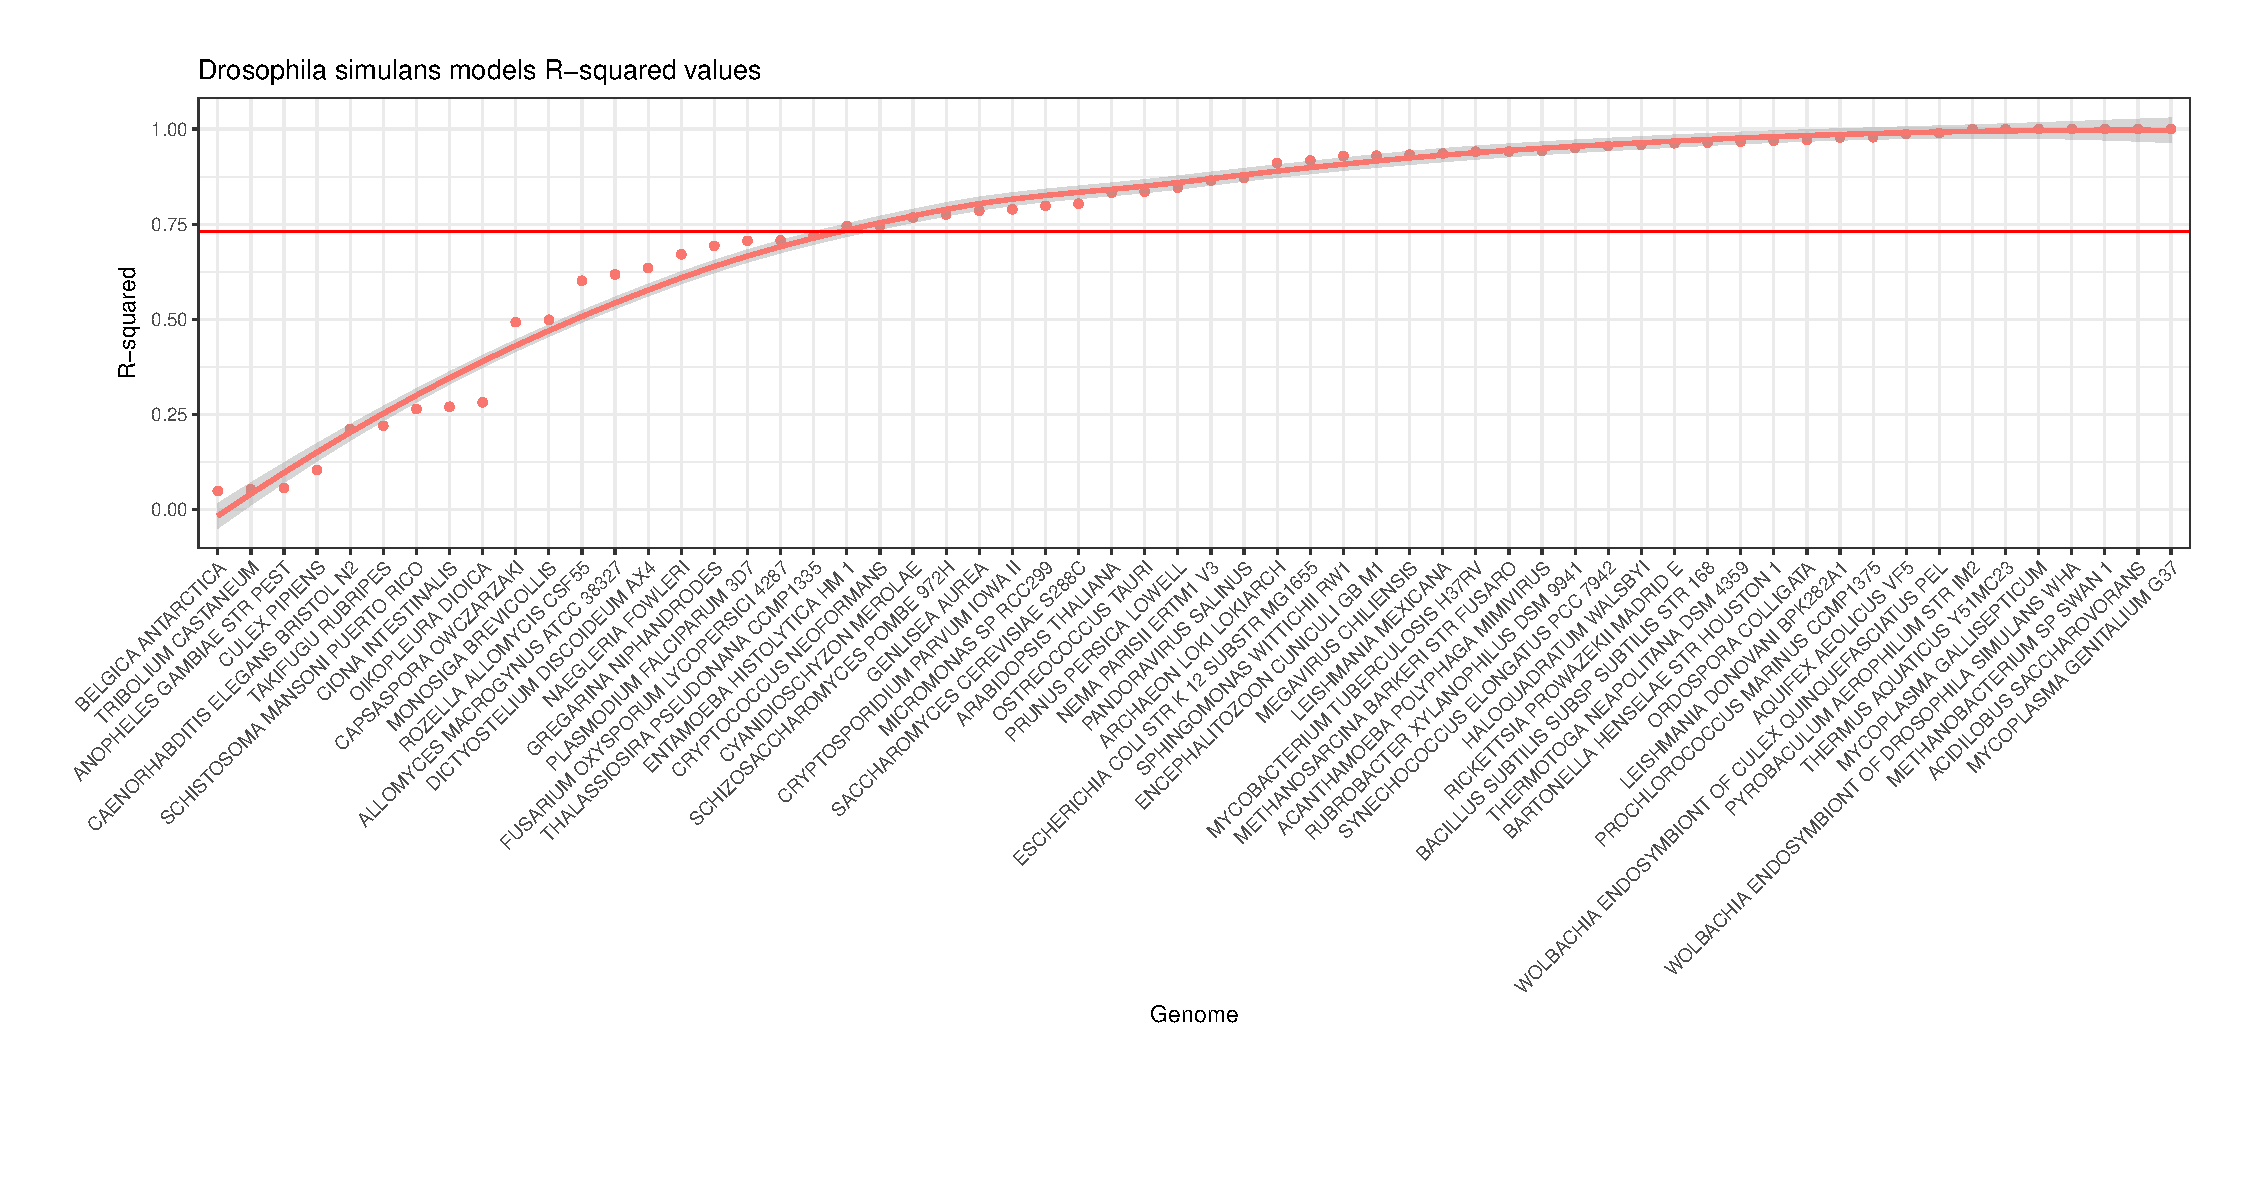
\includegraphics[width=12cm]{figures/rsq_drosoph_bootstrapped.pdf}
\caption{$R^2$ values for regression models for \textit{Drosophila} vs. all
other genomes.}
\label{fig:rsquared_curve}
\end{figure}
\end{center}
The majority of sequences (287942, 97.1\%) from each analyzed genome were
classified as core sequences in all metagenomic experiment with validated
regression models. 3992 (1.3\%) PPS were classified as "outsider" by one model
(in one comparison of two genomes). The remaining 4705 (1.6\%) sequences were
classified as “outsider multiple” and are the most likely candidates for HGT.
The list of protein-coding open reading frames classified as “outsider once”,
or “outsider multiple” along with their FASTA sequences is available for
download: [link]. For the fraction of “outsider once” and “outsider multiple”
genes varies from genome to genome see Supplement. An important limitation is
that our approach does not distinguish HGT from genomic contaminations. Thus
the observed differences in Core/Outsider ratio between different genomes, does
not necessarily indicate that some genomes are more prone to the acquisition of
sequences due to HGT. We used a PFAM analysis to check for any PFAM domains are
significantly overrepresented PPS that were classified as outsiders by some of
the models. A list of top-ranked findings (ranked by significance) is presented
in Table ~\ref{table:pfam_domains}. We would like to highlight some of the most
interesting findings.
\begin{center}
\begin{table}
{
	\setstretch{1}
\pgfplotstabletypeset[
    col sep=comma,
    string type,
    every head row/.style={%
        before row={\hline
            \multicolumn{2}{c}{Overrepresented PFAM Domains} & \\
        },
        after row=\hline
    },
    every last row/.style={after row=\hline},
    columns/pdom/.style={column name=PFAM Domain, column type=l},
    columns/spec/.style={column name=Species, column type=l},
    columns/pval/.style={column name=P-value, column type=c}
    ]{resources/pfam_domain_table.csv}
\caption{PFAM domains that are overrepresented among predicted horizontally
transferred protein-coding sequences}
\label{table:pfam_domains}
}
\end{table}
\end{center}

\subsection{Horizontal origin of Ankyrins in \textit{Wolbachia} endosymbiotic
bacteria}
\label{horizontal_origin}
Jernigan and Bordenstein \cite{Jernigan2014} showed that the lifestyle of
bacteria, rather than phylogenetic history, is a predictor of ANK repeat
abundance. They also showed that phylogenetically unrelated organisms that
forge facultative and obligate symbioses with eukaryotes show enrichment for
ANK repeats in comparison to free-living bacteria. This observation was
especially strong for obligate intracellular bacteria. Ankyrin domains are very
common in eukaryotes, but rare in bacteria, with the exception of parasites and
symbionts. In a paper by Siozios et al. \cite{Siozios2013} it is concluded that
ankyrin genes are likely to be horizontally transferred between strains with
the aid of bacteriophages. Al-Khodor et al. \cite{Al-Khodor2010} also suggests
that prokaryotic genes encoding ANK-containing proteins have been acquired from
eukaryotes by horizontal gene transfer. Coincidentally we independently
reproduced these findings: both species of endosymbiotic \textit{Wolbachia}
included in our study have genes encoding ANK-containing proteins acquired via
HGT by their ancestors according to our models.

\subsection{Horizontal origins of Taumatins in nematodes and insects}
Taumatins are a group of defensive proteins produced by plants in response to
fungal infections [link]. Recently the presence of these proteins was reported
in the desert locust \textit{Schistocerca gregaria}, one related species, and
in the nematode \textit{Caenorhabditis} but not in \textit{Drosophila} and
other insects \cite{Brandazza2004}. Our analysis suggests that the ancestors of
\textit{Caenorhabditis elegans} may acquired Thaumatin proteins via HGT.
According to InterPRO \cite{Finn2017} there are currently 4853 known Thaumatin
proteins (IPR001938). 3179 of them are found in land plants, 1120 in Fungi and
only 118 in Metazoa. The latter 118 are distributed among nematodes (59
proteins), panarthropods (57 proteins) and mollusks (2 proteins). This
distribution of Thaumatin proteins among the tree of life favors the idea that
HGT was involved in their evolution.

\subsection{HGT genes detected in Archaeon Loki}
Archaeon Loki was reported as a complex archaea that bridges the gap between
prokaryotes and eukaryotes \cite{Spang2015}. Our initial analysis revealed
sequences of one domains that is overrepresented among candidates for HGT in
Archaeon Loki: MaoC\_dehydratas. All 7 Maoc\_dehydratas containing proteins of
Archaeon Loki are not similar to any proteins found in archaea, but share some
degree of similarity to proteins found in d-proteobacteria according to a
simple BlastP search (e-values up to E-15).


\section{Conclusions}
We developed a novel approach capable of detecting candidate sequences for HGT.
Novel cases of putative HGT were identified in most studied species (excluding:
species name, species name, species name). We performed a systematic search for
PFAM domains that are highly overrepresented among them. The involvement of
some of these domains in HGT events has already been well-studied examples
of HGT, while others have not been reported before. We created a downloadable
database that contains all sequences, that were flagged as candidates for HGT.
Two important limitations of our approach should be noted: we are unable to
discern HGT from genomic contaminations using this method and the method is
computationally expensive.

\section{References}

\printbibliography
\end{document}
